%% LyX 2.2.1 created this file.  For more info, see http://www.lyx.org/.
%% Do not edit unless you really know what you are doing.
%\documentclass[english]{article}
%\usepackage[latin9]{inputenc}

%\usepackage{babel}
%begin{document}

\documentclass[english]{article}
\usepackage[T1]{fontenc}
\usepackage[latin9]{inputenc}
\usepackage[a4paper]{geometry}
\usepackage{amsmath}
\geometry{verbose,tmargin=0.5cm,bmargin=0.5cm,lmargin=0.5cm,rmargin=0.5cm}
\usepackage{graphicx}
%\usepackage[chapter]{algorithm}
\usepackage{algorithmic}

\DeclareMathOperator*{\argmin}{\arg\!\min}
\DeclareMathOperator*{\argmax}{\arg\!\max}

\makeatletter

%%%%%%%%%%%%%%%%%%%%%%%%%%%%%% LyX specific LaTeX commands.
%% Because html converters don't know tabularnewline
\providecommand{\tabularnewline}{\\}

\makeatother

\usepackage{babel}
\begin{document}

\title{Machine Learning for Computer Vision (EE5177) \\ Programming Assignment 1 : Fitting Probability Distribution to Data \\ Problem 1}

\author{Akshit Kumar \\ \emph{EE14B127}}

\date{5th February 2017}

\maketitle
\tableofcontents{}

\section{Calculation of ML, MAP and Bayesian Estimate}

\subsection{Goal}

We are given a set $X$ of $D$-dimensional data points generated
using a Gaussian distribution of mean $\mu$ and covariance matrix
$\Sigma$. We are also given the distribution of prior on the mean to
be a Gaussian with $P(\mu)=N_{\mu}(\mu_{o},\Sigma_{o})$. Given the
covariance, we are required to calculate the ML estimate of mean,
MAP estimate of mean and posterior distribution using Bayesian Methods.

\subsection{Calculation of ML Estimate of mean}

The Multivariate Gaussian Distribution is defined as : 

$$p(x|\mu,\Sigma)=\dfrac{exp\{\dfrac{-1}{2}(x-\mu)^{T}\Sigma^{-1}(x-\mu)\}}{\sqrt{|2\pi\sum|}}$$

Given a set of i.i.d data $X=\{x_{1},x_{2},x_{3},............................,x_{I}\}$
drawn from $N(x;\mu,\Sigma)$, we can estimate $(\mu,\Sigma)$ by \emph{Maximum
Likelihood Estimation}. The loglikelihood function is 

$$L=ln(p(x|\mu,\Sigma)=\dfrac{-I}{2}ln|\Sigma|-\dfrac{1}{2}\sum_{i}(x_{i}-\mu)^{T}\Sigma^{-1}(x_{i}-\mu)+ c$$

On taking derivative with respect to $\mu$ and setting to 0 gives : 

$$ \dfrac{dL}{d\mu}=\dfrac{-1}{2}\sum_{i}\dfrac{d(x_{i}-\mu)^{T}\Sigma^{-1}(x_{i}-\mu)}{d\mu}=0$$

$$ \dfrac{dL}{d\mu}=\dfrac{-1}{2}\sum_{i}(-2\Sigma^{-1}(x_{i}-\mu))=0$$

$$\implies \mu_{ML}=\dfrac{1}{I}\sum_{i}x_{i}$$

\subsection{Calculation of MAP Estimate of mean}
The Multivariate Gaussian Distribution is defined as : 

$$p(x|\mu,\Sigma)=\dfrac{exp\{\dfrac{-1}{2}(x-\mu)^{T}\Sigma^{-1}(x-\mu)\}}{\sqrt{|2\pi\sum|}}$$

We define the $\mu_{MAP}$ as follows 

$$ \mu_{MAP} = \argmax_{\mu}[\prod_{i=1}^{I}p(x_{i}|\mu,\Sigma)p(\mu)] $$
Similar to the \emph{Maximum Likelihood Estimate}, we can maximise the logarithm of the function, which implies
$$ \mu_{MAP} = \argmax_{\mu}[\sum_{i=1}^{I}log(p(x_{i}|\mu,\Sigma) + log(p(\mu))] $$

Let the cost function be $L = \sum_{i=1}^{I}log(p(x_{i}|\mu,\Sigma) + log(p(\mu)) $
It can be simplied as 
$$ L = \sum_{i=1}^{I}(x_{i}-\mu)^{T}\Sigma^{-1}(x_{i}-\mu) + (\mu - \mu_{o})^{T}\Sigma_{o}{-1}(\mu - \mu_{o}) $$
On differentiating L with respect to $\mu$ and setting to 0, we get :
$$ \dfrac{dL}{d\mu} = \sum_{i=1}^{I}\Sigma^{-1}(x_{i} - \mu) + \Sigma_{o}^{-1}(\mu - \mu_{o}) = 0$$
On re-arranging the terms, we get:
$$ \implies (I\Sigma^{-1} + \Sigma_{o}^{-1})\mu_{MAP} = \sum_{i=1}^{I}\Sigma^{-1}x_{i} + \Sigma_{o}^{-1}\mu_{o} $$
$$ \implies \mu_{MAP} = (I\Sigma^{-1} + \Sigma_{o}^{-1})^{-1}(\sum_{i=1}^{I}\Sigma^{-1}x_{i} + \Sigma_{o}^{-1}\mu_{o}) $$

\subsection{Calculation of Posterior Distribution using Bayesian Method}
As given in the question, we assume that $p(x|\mu) = N(\mu,\Sigma)$ and $p(\mu) = N(\mu_{o},\Sigma_{o})$ where $\Sigma$, $\Sigma_{o}$ and $\mu_{0}$ are known. After observing a det $D$ of $n$ independent samples $x_{1},x_{2},...........,x_{n}$, we use the Bayes' Theorem to obtain

$$ p(\mu|D) = \alpha\prod_{i=1}^{n}p(x_{i}|\mu)p(\mu) $$
$$ p(\mu|D) = \beta \exp[\dfrac{-1}{2}(\mu^{T}(n\Sigma^{-1} + \Sigma_{o}^{-1})\mu - 2\mu^{T}(\Sigma^{-1}\sum_{i=1}^{n}x_{i} + \Sigma_{o}^{-1}\mu_{0}))] $$ ,which has the form 
$$ p(\mu|D) = \gamma \exp[\dfrac{-1}{2}(\mu - \mu_{n})^{T}\Sigma_{n}^{-1}(\mu - \mu_{n})] $$
Thus we can say that $p(\mu|D) = N(\mu_{n},\Sigma_{n})$ where we have
$$ \mu_{n} = \Sigma_{o}(\Sigma_{o} + \dfrac{1}{n}\Sigma)^{-1}\mu_{n}^{*} + \dfrac{1}{n}\Sigma(\Sigma_{o} + \dfrac{1}{n}\Sigma)^{-1}\mu_{o} $$
$$ \Sigma_{n} = \Sigma_{o}(\Sigma_{o} + \dfrac{1}{n}\Sigma)^{-1}\dfrac{1}{n}\Sigma $$
Observe that $x$ can be viewed as the sum of two mutually independent random variables, a random vector $\mu$with $p(\mu|D) = N(\mu_{n},\Sigma_{n})$ and an independent random vector $y$ with $p(y) = N(0,\Sigma)$. Since the sum of two independent, normally distributed random vectors is again a normally distributed vector whose mean is the sum of the means and whose covariance matrix is the sum of covariance matrices. we have $$p(x|D) = N(\mu_{n},\Sigma + \Sigma_{n})$$

\section{Plots of Bhattacharya Distance of ML,MAP and Bayesian}
\subsection{Goal}
The estimates derived using Maximum Likelihood, Maximum A Posteriori and Bayesian Methods can be analysed quantitatively using the Bhattacharya distance as a distance metric between the ground truth values and the estimated values.

\subsection{Plot of ML and MAP for Prior-1}
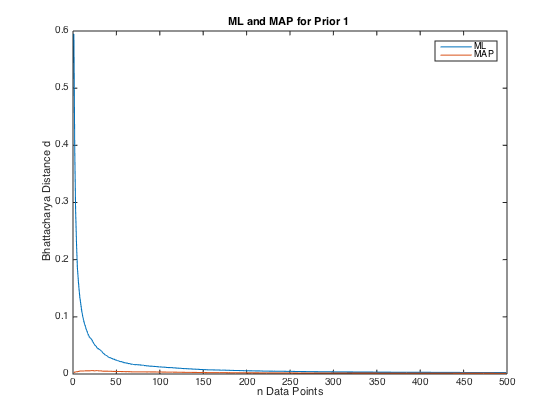
\includegraphics[scale=0.8]{plot1}


\subsection{Plot of MAP and Bayesian for Prior-1}
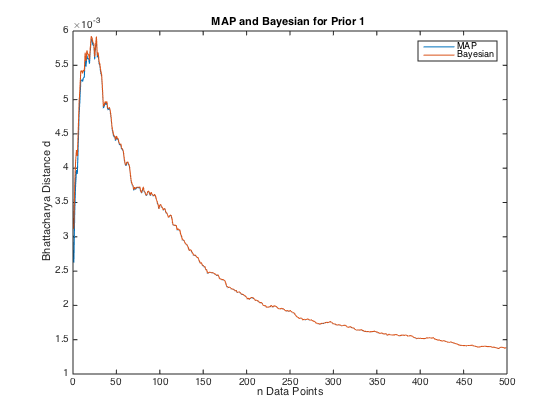
\includegraphics[scale=0.8]{plot2}


\subsection{Plot of ML and MAP for Prior-2}
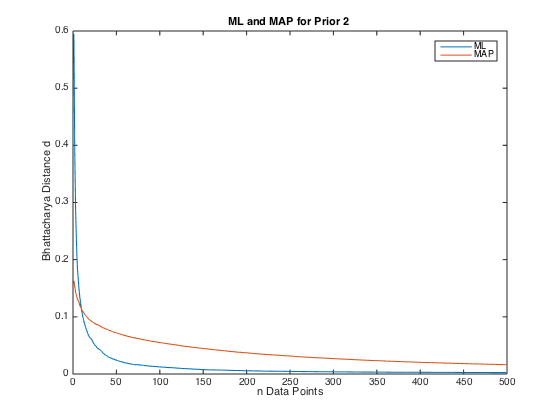
\includegraphics[scale=0.8]{plot3}

\subsection{Plot of MAP and Bayesian for Prior-2}
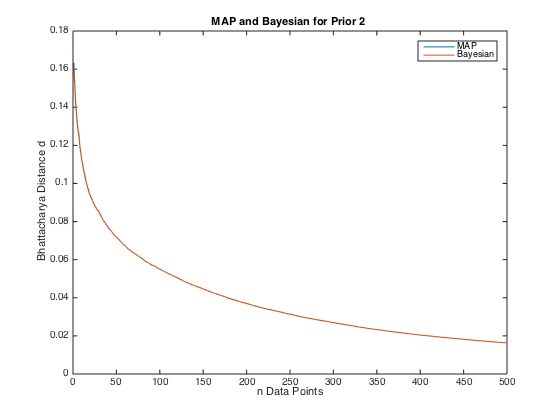
\includegraphics[scale=0.8]{plot4}

\section{Inferences}
\subsection{Comparison of ML and MAP estimate from $d$ vs. $n$ plots}
From the $d$ vs. $n$ plot for Prior-1 shows that initially ML estimate is worse compared to MAP estimate but as n increases, the ML estimate converges to the MAP estimate,performing as well as MAP estimate as n increases(goes to 500).Since the MAP estimate is so low to start with, it implies that Prior-1 is close to the true prior.\newline
From the $d$ vs. $n$ plot for Prior-2 shows that initially ML estimate is worse compared to MAP estimate, for some 20 odd iterations and then after that quickly converges to the true value, performing better than the MAP estimate. The plot shows that MAP estimate will require a lot data to converge to the true values of the mean and covariance.

\subsection{Comparison of MAP and Bayesian estimate from $d$ vs. $n$ plots}
From both the plots, the MAP and the Bayesian estimates seem to be performing the same as the plot for MAP and Bayesian overlap with each other. 
\newline
For prior-1, MAP and Bayesian estimates both increase initially and start decreasing after some 50 odd points. 
\newline
For prior-2, MAP and Bayesian estimates continuously decrease as n increases but lot of data points to converge to the true values.

\end{document}
